\begin{chapter}{Kapitel}
 \section*{Chapter 2.1}
 
 \f{Verifikation}: \ku{check that we are building the thing right}
 \vspace*{3pt}
 
 \noindent Soll den Nachweis liefern, dass das System die Anforderungen immer erfüllt (Korrektheit der Implementierung in Bezug auf die Spezifikation).
 \vspace*{3pt}
 
 \f{Validation}: \ku{check that we are building the right thing}
 \vspace*{3pt}
 
 \noindent Entspricht eher dem kritischen Überprüfen der Spezifikation anhand eines ersten Designs auf Richtigkeit und Vollständigkeit.
 
 \f{Testen}: \ku{ist ein Mittel für beides und weit verbreitet.}
 \vspace*{3pt}
 
 \noindent Verifikation lässt sich damit nicht bewerkstelligen, allenfalls Falsifikation. 
 \vspace*{8pt}
 
 \f{Populäre Techniken der Verifikation}:
\begin{itemize}
 \item \f{Peer Reviewing}: Statische Methode der manuellen Durchsicht und Prüfung des Codes durch einen Experten. Im Mittel bringt dies 60\% der Fehler, subtile
 Fehler werden meist nicht gefunden.
 \item \f{Testen}: Dynamische Methode, häufig unterstützt durch Qualitätsmetriken (Code Coverage). 30\% bis 50\% der Gesamtkosten gehen auf das Konto von Testen, 
 bei Hardware sind oft 70\% des entwickelten Codes Testbenches.
\end{itemize}
Man kann mit Tests die Anwesenheit von Fehlern nachweisen, nicht jedoch deren Abwesenheit!
\vspace*{8pt}

\f{Formale Methoden}:
\vspace*{4pt}

\noindent Formale Methoden basieren auf formalen Sprachen zur Spezifikation von Eigenschaften wie auch zur Konstruktion des Systems. Gebräuchliche 
Verifikationstechniken mit formalen Methoden sind:
\begin{itemize}
 \item \f{Deduktive Methoden}: Hier liefert man einen mathematischen Beweis, dass die Implementierung die Spezifikation erfüllt. Meist werden Theorembeweiser 
 oder Beweisprüfer als Werkzeuge benutzt. Problem: Sehr aufwändig, das System muss die Form einer Mathematischen Theorie haben.
 \item \f{Model Checking}: Systematische und erschöpfende Überprüfung der Spezifikation auf allen erreichbaren Systemzuständen. Meist vollautomatisch durch 
 sogenannte Modellchecker. Problem: Zustandsraumexplosion
 \item \f{Modelbasierte Simulation und Test}: Exploration möglicher Verhalten mit Überprüfung der Spezifikationen
\end{itemize}

\f{Model-Checking}:
\vspace*{4pt}

\noindent Man betrachtet 
\begin{itemize}
 \item \f{Spezifikation}: formale Definition der Eigenschaften des gewünschten Systems in Form von Sätzen einer mathematischen Theorie (Aussagen einer temporalen 
 Logik)
 \item \f{Implementierung}: formale Definition der konkreten Konstruktion des Systems (als diskretes Transitionssystem)
 \item \f{Model Checking}: Ist die Implementierung ein Modell für die Theorie (gelten die Sätze für die Implementierung)
\end{itemize}
\begin{figure}[!ht]
 \centering
 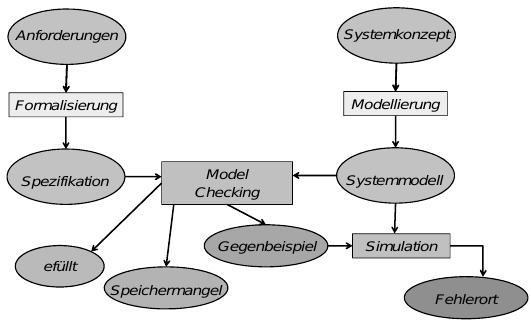
\includegraphics[scale=0.8]{pics/modelchecking}
\end{figure}

\f{Transitionssysteme}:

\f{Definition}: \ku{Ein Tupel $T=(S,(Act,)\rightarrow, St)$ heißt Transitionssystem, wobei}
\begin{itemize}
 \item $S$ \dots eine Menge von Zuständen 
 \item $\rightarrow \subseteq S\times S$ die Transitionsrelation ($\rightarrow \subseteq S\times Act \times S$)
 \item $Act$ eine Menge von Aktionen 
 \item $ST \subseteq S$ eine Menge von Startzuständen ist 
\end{itemize}

\noindent Auf die Startzustände kann man auch verzichten oder auf genau einen gehen, der dann vermöge $\rightarrow$ nichtdeterministisch in $St$ verzweigt.
\vspace*{4pt}

\noindent Auch die Aktionen sind Komfort, sie machen es leichter, mehrere kooperierende Transitionssysteme zu definieren und Synchronisationsbedingungen über Aktionen zu 
formulieren. Wenn wir die Zustandsmenge endlich machen und die Aktionen als Ein/Ausgabemarkierungen auffassen, sind wir wieder bei unseren vertrauten Automaten.
\vspace*{4pt}

\noindent Bei endlicher Zustandsmenge ist auch klar, dass man die Übergangsrelation als gerichteten Graphen darstellen kann. 
\begin{figure}[!ht]
 \centering
 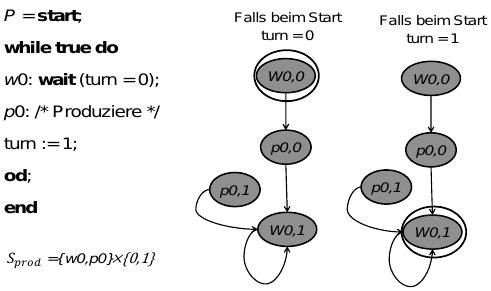
\includegraphics[scale=0.8]{pics/transitionssystem}
 \caption{Producer als Transitionssystem}
\end{figure}

\f{Kripke-Strukturen}:
\vspace*{4pt}

\noindent Praktisch stellt man Eigenschaften eines Systems durch Messung fest, d.h. Eigenschaften sind im einfachsten Falle binär, sie gelten oder gelten nicht.
\vspace*{4pt}

\noindent Alles was wir über das Verhalten eines System wissen oder erfahren können sollte sich also grundsätzlich gesehen auf endlich viele (wir können nur endlich viel 
messen) \f{atomare Aussagen} zurückführen lassen. Wir erweitern ein Transitionssystem zu einer \f{Kripke Struktur}: 

\[K = (S,(Act,)\rightarrow, St, AP, L)\]

\noindent Dabei kommen noch zwei Komponenten dazu: 
\begin{itemize}
 \item $AP$ \dots eine (endliche) Menge von atomaren Aussagen (atomic propositions)
 \item $L:S \rightarrow 2^{AP}$ \dots eine Markierung der Zustände mit den durch sie erfüllten atomaren Aussagen (labeling) 
\end{itemize}

\newpage 
\noindent Das Transitionssystem zu den Producer/Consumer-Prozessen könnte man durch folgende atomare Aussagen erweitern: \[AP=\{p,k\}\] mit $p$: es wird gerade produziert 
\\ und $k$: es wird gerade konsumiert
\vspace*{5pt}

\f{Linear-Zeit vs. Baum-Zeit}:
\vspace*{5pt}

\noindent Formal werden wir zu verifizierende Eigenschaften unserer Systeme in \f{temporaler Logik} ausdrücken. 
\vspace*{4pt}

\noindent Die \f{Linear-Zeit Logik (linear time logic, LTL)} erlaubt Aussagen über Labelings aller (unendlichen) Berechnungsfolgen der Kripke-Struktur. 
LTL-Aussagen gelten entweder für alle Folgen oder nicht. 
\vspace*{4pt}

\noindent Die \f{Baum-Zeit Logik (computation tree logic, CTL)} erlaubt die Formulierung von Aussagen über Berechnungsbäume, d.h. man kann Existenz und 
Allquantoren für die Pfade in den Unterbäumen nutzen.

\section*{Chapter 2.2}
\f{Linear-Time Logic} 
\vspace*{3pt}

\noindent Linear-Zeit Logik ist eine Logik, die auf Sequenzen von Belegungen mit atomaren Eigenschaften basiert. Die Zeit ist diskret und schreitet linear voran. Es gibt 
nur eine mögliche Zukunft.
\vspace*{4pt}

\noindent Sei $AP$ die Menge der atomaren Aussagen. Dann korrespondiert das Labeling $X \subseteq AP$ zu der Tatsache, dass alle Eigenschaften $x\in X$ in dem 
Zustand gelten und alle $y\in AP\setminus X$ in diesem Zustand nicht gelten.

\noindent LTL Formeln werden nun über Mengen von unendlichen Folgen von Labelings interpretiert. D.h. wir betrachten Sequenzen $\sigma \in (2^{AP})^\omega$, wofür
ein Alphabet $\Sigma, \Sigma^\omega$ die Menge aller unendlichen Folgen über $\Sigma$ sei. 

\noindent Für $\sigma \in (2^{AP})^\omega$ sei 
\begin{itemize}
 \item $\sigma(i) \subseteq AP$ das i-te Element der Folge
 \item $\sigma^i \in (2^{AP})^\omega$ die unendliche Folge $\sigma(i)\sigma(i+1)\sigma(i+2)\dots$
\end{itemize}

\f{Syntax von LTL}

\noindent Sei $AP$ eine Menge von atomaren Aussagen. Dann ist die Menge der LTL Formeln über $AP$ wie folgt definiert: 
\begin{enumerate}
 \item jedes $p\in AP$ ist eine LTL Formel 
 \item sind $\Phi_1$ und $\Phi_2$ Formeln, dann auch $\neg \Phi_1$, $\Phi_1 \bigvee \Phi_2$, $\f{X}\Phi_1$, $\Phi_1\f{U}\Phi_2$
 \item nichts sonst ist eine LTL Formel 
\end{enumerate}

\noindent Dies ist eine sehr minimalistische Definition. \f{X} (next) und \f{U} (until) sind temporale Operatoren. 
\vspace*{4pt}

\noindent LTL Formeln werden über (unendlichen) Folgen von Teilmengen atomarer Aussagen interpretiert. Die Semantik einer LTL-Formel $\Phi$ ist die Menge aller 
Folgen $\sigma \in (2^{AP})^\omega$, die $\Phi$ erfüllen, d.h. 
\[[[\Phi]] = \{\sigma | \sigma \vDash \Phi\}\]

\f{Erfüllung einer LTL-Formel}

\noindent Sei $\sigma \in (2^{AP})^\omega$ und sei $\Phi$ eine LTL Formel. Dann gilt $\sigma \vDash \Phi$ (``$\sigma$ erfüllt $\Phi$'') nach folgender
Fallunterscheidung über die Struktur von $\Phi$:
\begin{itemize}
 \item $\sigma \vDash p$ \qquad \qquad   falls $p\in AP$ und $p\in\sigma(0)$
 \item $\sigma \vDash \neg\Phi$ \qquad  \qquad falls $\sigma \nvDash \Phi$
 \item $\sigma \vDash \Phi_1 \bigvee \Phi_2$ \qquad falls $\sigma \vDash \Phi_1$ oder $\sigma \vDash \Phi_2$
 \item $\sigma \vDash \f{X}\Phi$ \qquad  \qquad falls $\sigma^1 \vDash \Phi $
 \item $\sigma \vDash \Phi_1\f{U}\Phi_2$ \qquad falls $\exists i: \left(\sigma^i\vDash \Phi_2 \wedge \forall k < i:\sigma^k \vDash \Phi_1 \right)$
\end{itemize}


\end{chapter}
